\documentclass[conference]{IEEEtran}

\usepackage[T1]{fontenc}
\usepackage{amsmath,amssymb}
\usepackage{booktabs}
\usepackage{graphicx}
\usepackage{microtype}
\usepackage{xcolor}
\usepackage{url}

\begin{document}
\setcounter{page}{5}
\setcounter{section}{7}
\setcounter{equation}{10}
\setcounter{figure}{4}
\setcounter{table}{5}

\section{Implementation Contracts and Edge Semantics}
Reproducibility requires more than a high-level algorithm name. Each public
class validates two-dimensional finite input, stores the observed feature
count, preserves original class labels, and raises an explicit pre-fit error.
The tree exposes depth and leaf count as properties and importance as the
method required by the brief; the forest exposes aggregate importance as a
property. Predictions always return the original label dtype. Probabilities
follow sorted global class order and sum to one, including when a bootstrap
tree observes only a strict subset of classes.

\subsection{Tree Search Invariants}
At a node containing $n_v$ rows and $p_v$ candidate features, stable sorting
costs $O(p_v n_v\log n_v)$ and a complete threshold scan costs
$O(p_v n_v K)$ only for the vector impurity arithmetic. Empty-weight children
are rejected even if they contain zero-weight rows. This distinction matters:
sample count governs structural stopping, while total positive weight governs
the split objective and leaf distribution. Multiplying every sample weight by
a positive constant cannot change a split.

The test matrix checks one feature, all one class, noncontiguous and string
labels, repeated values, constant features, deterministic equal-gain features,
zero-weight observations, entropy, feature subsampling, and root depth zero.
XOR is retained as a conceptual defense case. A greedy impurity tree correctly
halts because neither root feature has positive gain; depth alone does not add
look-ahead. The limitation helps explain why additive stumps can create a more
expressive boundary over rounds even though one stump cannot solve the task.

\subsection{Ensemble State and Numerical Safety}
AdaBoost stores only accepted estimators. Its estimator error array contains
the unclipped observed errors, while clipping is restricted to logarithms and
weight updates. A first learner at or beyond the class-aware random threshold
raises a clear error; a later rejected learner ends the sequence and leaves the
previous valid ensemble usable. For SAMME.R, probability floor
$10^{-12}$ prevents $\log 0$ and centered log-probabilities prevent a common
offset from changing class preference. Stable softmax subtracts each row
maximum.

Forest bootstrap and tree seeds come from independent children of one
\texttt{SeedSequence}; workers never inherit mutable RNG state. The complete
bootstrap array and its exact OOB complement are retained. A forest with OOB
scoring disabled does not silently expose a meaningless score, and requesting
OOB with \texttt{bootstrap=False} is invalid. Prediction ties resolve through
global class order, matching the deterministic tree rule.

\begin{table}[t]
\caption{Binding interfaces and principal fitted evidence.}
\centering
\begin{tabular}{lp{4.7cm}}
\toprule
Class & Principal fitted state \\
\midrule
DecisionTree & \texttt{classes\_}, root, depth, leaves, importances \\
AdaBoost & stumps, estimator weights/errors, stages \\
Random Forest & trees, bootstrap/OOB indices, coverage/score \\
PCA & training mean, ordered components, variance ratios \\
K-Means & centroids, labels, inertia, iteration count \\
DBSCAN & labels, core-sample indices \\
\bottomrule
\end{tabular}
\end{table}

\subsection{Clustering Details}
K-Means final inertia is recomputed after the final centroid update, preventing
a mismatch between stored labels, centroids, and objective. When duplicate
points make a cluster empty, the row with largest current residual is selected
deterministically and cannot be reused for two simultaneous empty clusters.
DBSCAN precomputes inclusive squared neighborhoods. Expansion uses a queue and
a membership flag so duplicate neighbor discoveries do not cause unbounded
work. A row marked noise before another core point is expanded can be relabeled
as border, matching reachability semantics.

\section{Complete Experiment Evidence Contract}
Each required experiment preserves raw units---stage, fold, replicate,
depth, bootstrap model, or cluster configuration---before a plot or summary is
made. This prevents a polished average from becoming the only surviving
evidence.


\subsection{Hypotheses Before Observing Results}
The experiments were designed around falsifiable expectations rather than a
post-hoc search for favorable plots. Increasing AdaBoost stages should first
reduce training error monotonically or nearly so; test error may bottom out if
later stumps focus on ambiguous samples. Increasing forest size should reduce
the variability of test and OOB estimates, with diminishing returns once the
correlated component in~(8) dominates. Increasing depth should reduce bias but
increase individual-tree variance; bootstrap averaging may tolerate deeper
trees than a single-tree baseline.

Noise creates a mechanism-specific contrast. AdaBoost can amplify mislabeled
rows through repeated error weighting. A forest never shares sample weights
across trees and therefore distributes the damage over bootstrap samples, but
deep trees can still memorize corrupt labels. Consequently, ``forest is always
more robust'' is not treated as a theorem; replicate uncertainty and data
geometry determine the observed conclusion.

Severe imbalance poses a different risk. Accuracy can remain high while a rare
class is never predicted, so macro F1 and macro OVR AUC are mandatory. Training-
fold oversampling improves the chance that rare classes influence a split, but
can increase variance through repeated rows. Because the test distribution is
untouched, the evaluation remains a test of population-like performance rather
than an artificially balanced target.

\begin{figure}[t]
\centering
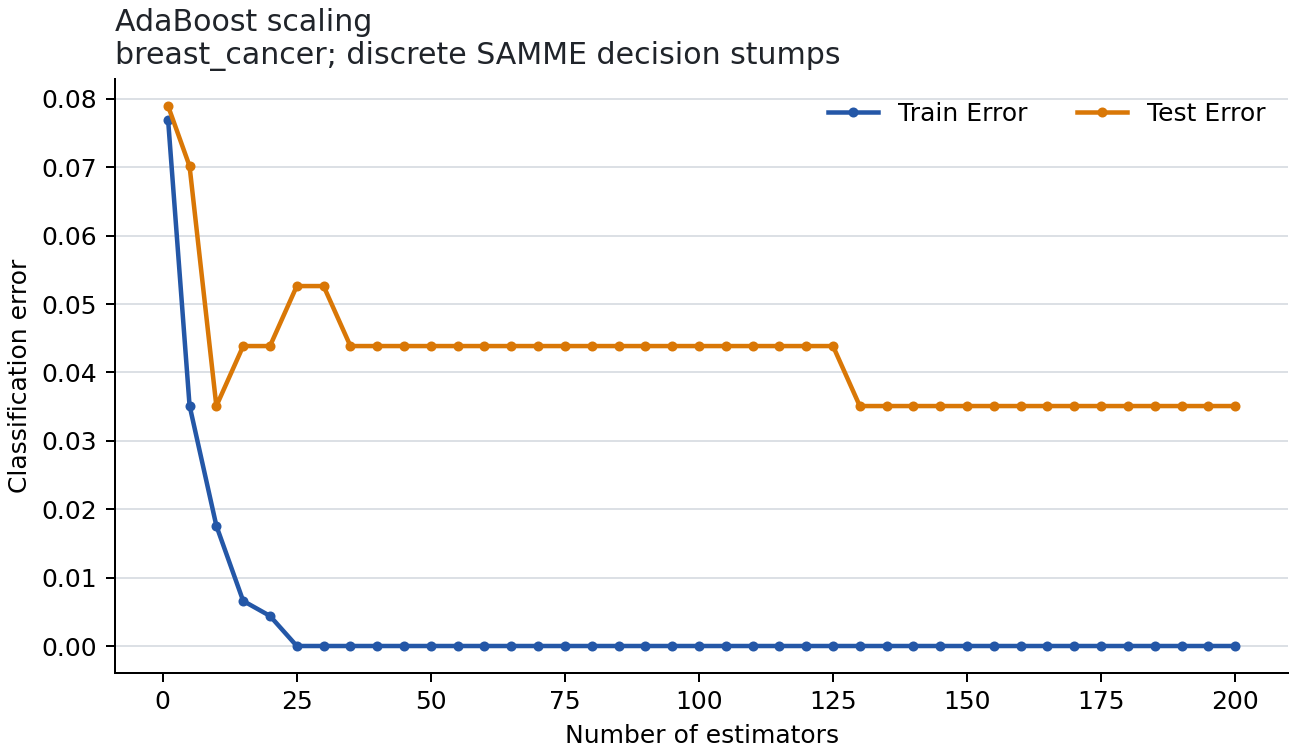
\includegraphics[width=\columnwidth]{../figures/02_adaboost_scaling/breast_cancer.png}
\caption{Full staged AdaBoost curve through 200 accepted rounds unless early
stopping occurs.}
\end{figure}

\begin{figure}[t]
\centering
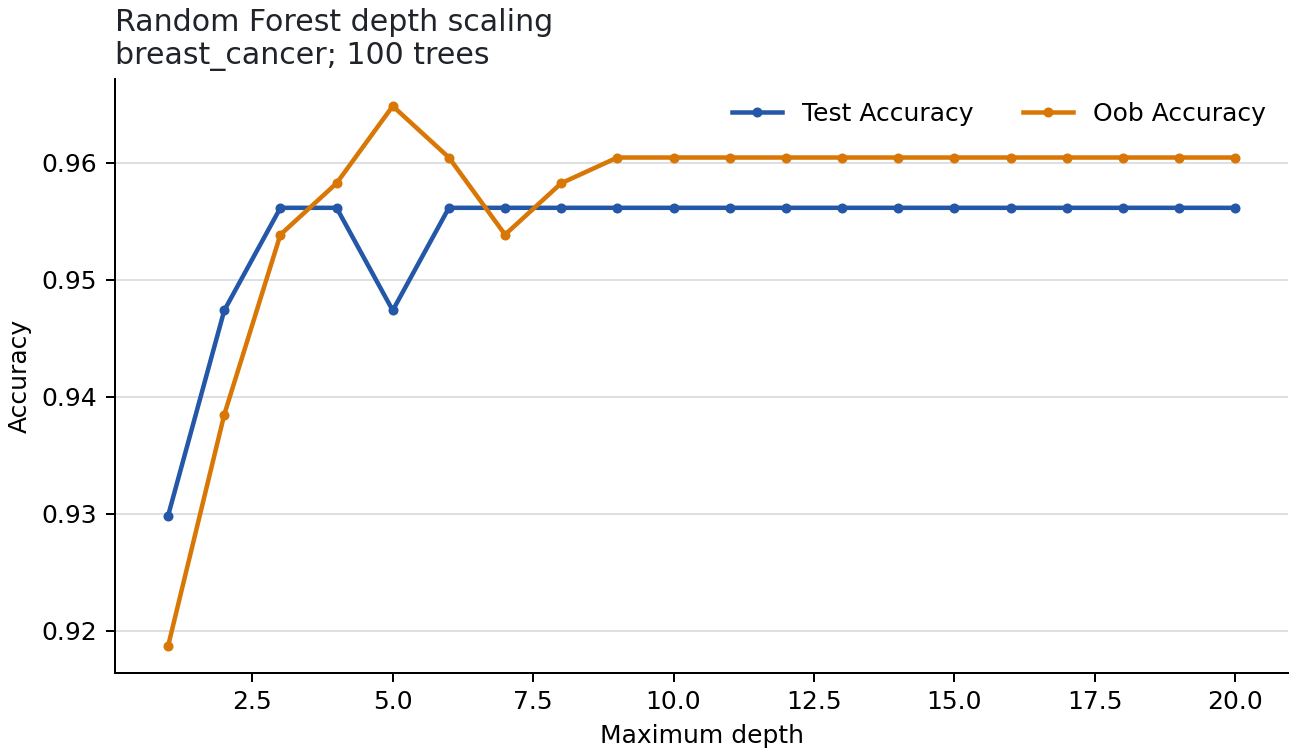
\includegraphics[width=\columnwidth]{../figures/03_rf_scaling/breast_cancer_depth.png}
\caption{Full depth sweep with separate OOB and clean-test accuracy.}
\end{figure}

\subsection{Complexity and Resource Strategy}
The implementation intentionally prioritizes clarity, but avoids the most
expensive naive operations. Tree class counts are incremental; staged
AdaBoost predictions reuse one maximum fit; Random Forest size curves reuse
prefixes of one 200-tree forest; distances used by DBSCAN and the $k$-distance
plot are computed only on a deterministic visualization sample. Bias--variance
probabilities are compressed to NPZ rather than serialized model by model.
The completed full run required 6.88 hours. Its manifest, generated artifacts,
and validation trail retain the exact configuration and numerical evidence
needed for audit without changing model seeds or metrics.

\section{Bonuses, Threats to Validity, and Defense Readiness}
\subsection{Gradient Boosting Extension}
The bonus classifier uses binary labels $y_i\in\{0,1\}$ and an initial raw
score $F_0=\log[\bar y/(1-\bar y)]$. At stage $m$, probabilities are
$p_i=\sigma(F_{m-1}(x_i))$ and the negative log-loss gradients are
\begin{equation}
r_{im}=y_i-p_i. \label{eq:gradient}
\end{equation}
A shallow from-scratch regression tree fits $r_{im}$ by midpoint splits that
minimize child squared error. The update
$F_m(x)=F_{m-1}(x)+\eta h_m(x)$ uses a stable sigmoid for both signs of $F$.
Training log loss is stored after every stage, and tests require a decreasing
trend, finite normalized probabilities, and equality between the last staged
prediction and the final prediction. The method is intentionally binary; a
multiclass extension is outside the claimed bonus scope.

\subsection{PCA Versus t-SNE}
PCA is deterministic, linear, and provides explained-variance accounting.
t-SNE uses a fixed stratified sample, PCA initialization, automatic learning
rate policy, recorded perplexity, and seed 42. It supplies a complementary
local-neighborhood view, not a clustering score. Apparent separation can vary
with perplexity and random optimization; distant point-to-point distances,
cluster area, and relative inter-group spacing are therefore excluded from the
argument. K-Means and DBSCAN remain evaluated in the retained PCA space.

\begin{figure}[t]
\centering
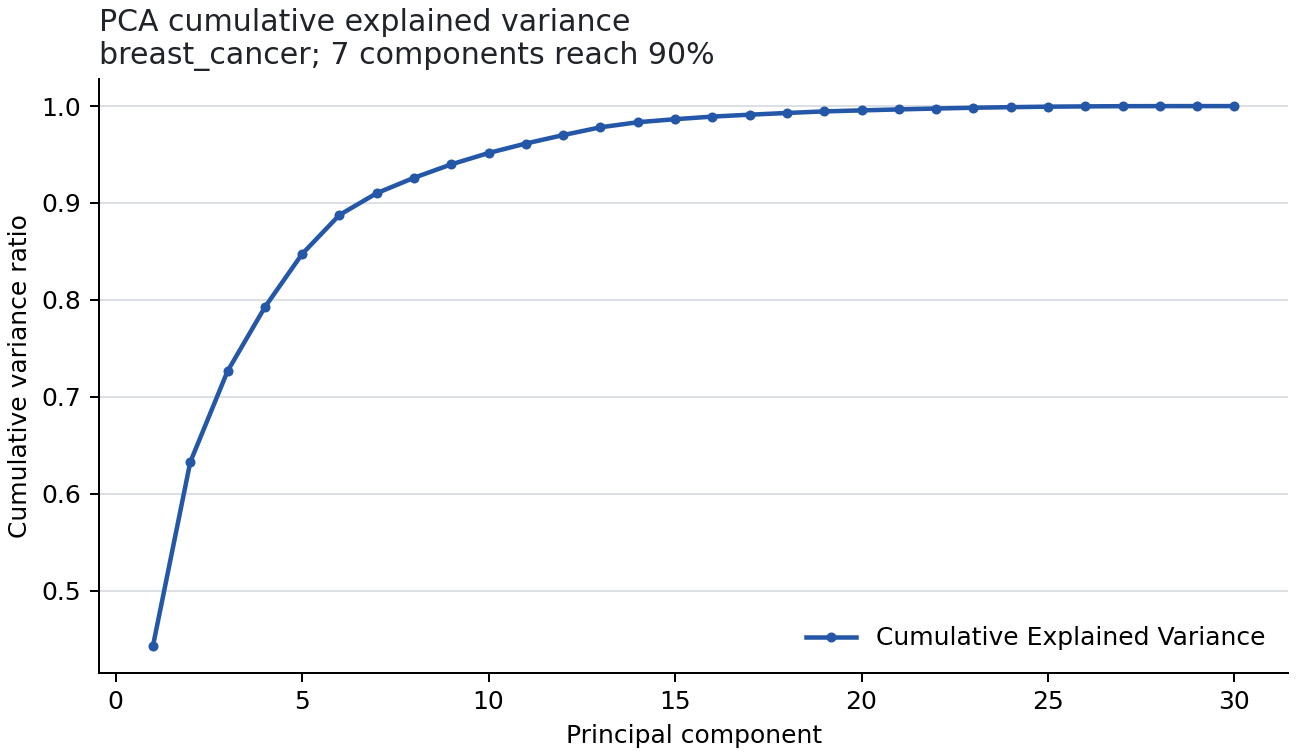
\includegraphics[width=\columnwidth]{../figures/07_unsupervised/breast_cancer_scree.png}
\caption{Cumulative variance provides a reproducible dimensionality rule.}
\end{figure}

\begin{figure}[t]
\centering
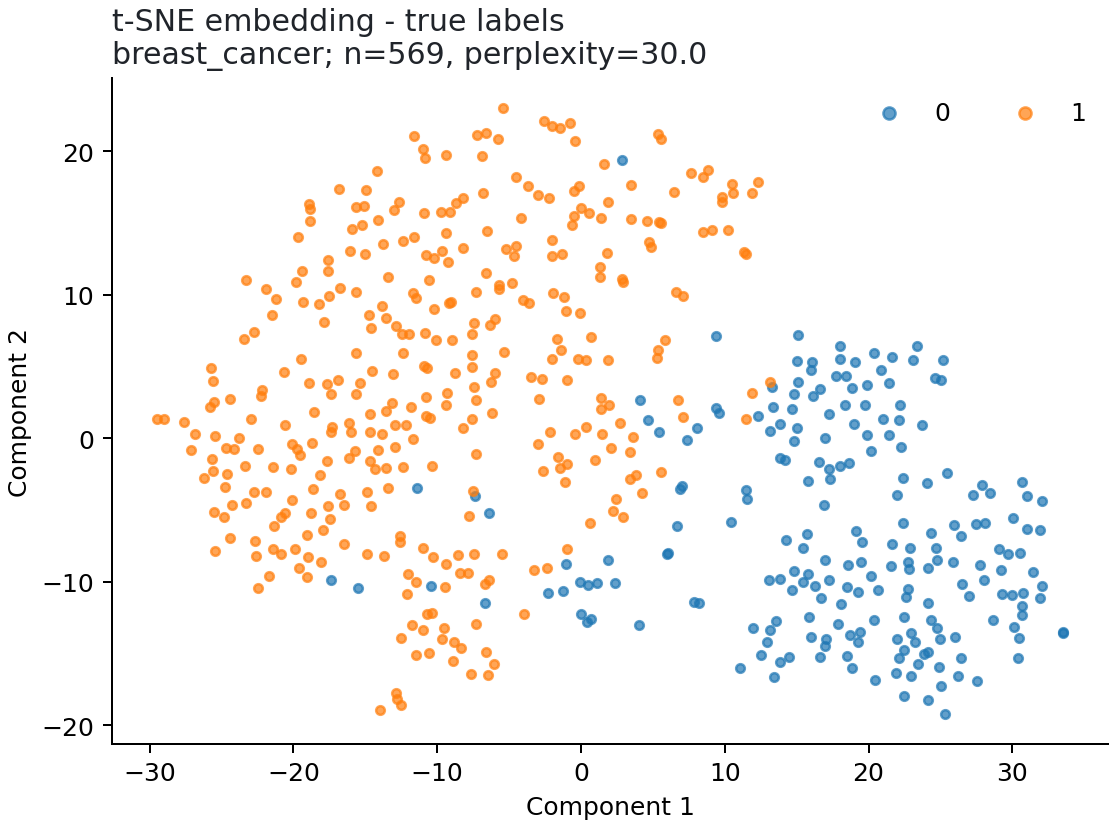
\includegraphics[width=\columnwidth]{../figures/bonus_tsne/breast_cancer.png}
\caption{t-SNE is a local visualization bonus and is not used to assert global
metric cluster structure.}
\end{figure}

\subsection{Threats to Internal and External Validity}
Reference agreement establishes a useful implementation check but does not
prove identical behavior: tie rules, stopping tolerances, category treatment,
and probability conventions can differ. To reduce this threat, correctness is
also tested with hand-computed cases and invariants. Fixed seeds improve audit
repeatability but do not represent uncertainty; cross-validation, five noise
replicates, and 100 bootstrap replicates supply the required variation.

Dataset conclusions are not universal. Breast Cancer is small and mostly
continuous; Adult has mixed socioeconomic features and missing categories;
Covertype is larger, multiclass, high-dimensional, and severely imbalanced.
The three together vary important factors, but they do not span concept drift,
adversarial noise, image structure, or calibrated-risk applications. The
project therefore reports conditional findings tied to source versions and
realized samples.

Bias--variance estimates use a finite fixed test set. They answer how fitted
probabilities vary across bootstrap training samples at those points, not the
entire population expectation. The reported decomposition residual checks
algebra, while it cannot remove sampling uncertainty. Similarly, OOB accuracy
is based only on covered rows and is not identical to five-fold CV.

\subsection{Defense and Release Gates}
Each primary module has a different reviewer and a backup owner. Defense drills
cover the derivation and code location of weighted impurity, SAMME's
$\log(K-1)$ term and rejection threshold, the correlation term in forest
variance, OOB coverage, PCA centering, K-Means empty clusters, and DBSCAN's
noise-to-border transition. A member claiming work must substantiate it with a
real commit, review, experiment run, report edit, or slide contribution.

The release gate requires all tests, at least 85\% measured coverage, clean
Ruff and mypy output, a successful no-argument full experiment run, dataset
constraint assertions, a valid executed notebook, six content pages plus
references, a 10--12 slide rendered deck, an all-member-approved contribution
report, and an auditable Git history. Only then is \texttt{v1.0-final} created
and the exact tagged artifacts uploaded to Moodle.

\end{document}
